\chapter{Internet measurement with RIPE Atlas}
\label{sec:ripe_atlas}
\section*{Abstract}
Starting from this chapter, the center of our study is oriented to delay and path measurements, and how to make use of them in measurement-based interdomain \ac{TE}.
Same as volume statistics studied in Chapter~\ref{sec:pref_selec}, these measurements are readily available on client TE platforms.
However, we decided to switch to measurements collected by RIPE Atlas, a measurement platforms offering open access to public, for the sake of reproducibility.
This decision is justified through a brief analysis on the elements of reproducibility and how RIPE Atlas satisfies then in design.
To facilitate the discussion in later chapter concerning measurement collection, we introduce succinctly the building blocks of RIPE Atlas, its measurement methods and how a certain set pf measurements can be identified and retrieved.

RIPE Atlas is a great facilitator for a better understanding of the Internet, yet it is not without out problems. We studied as well the potential data quality issues stemmed from the platform itself, as well as those specific to the our study on inter-domain TE.
At the end of this chapter, we present a case study that inspires the remaining research in this thesis.
\clearpage

\section{Reproducibility}
\marginpar{Issue with previous dataset.}
We collected traffic volume and delay data from real client networks in Section~\ref{sec:pref_selec} and developed all the studies concerning prefix selection on that dataset.
Having access to real client data increases the credibility of the discoveries made in the study, and enhances the relevance of proposed schemes basing on these findings.
The other side of coin is that such private dataset hinder the reproducibility, a paramount feature in metrology researches.

\marginpar{What we talk about when we talk about reproducibility?}
The \acf{ACM} offers definition for various terms referring to different degrees of research repoducibility~\cite{acm}, ranging from repeating the same result by the same team to reproducing the same result with independent implementation of proposed methods or measurement system.
The way the measurement data is generated, stored and accessed is one of the key elements for all these degrees of reproducibility.

\marginpar{data generation}
Previous data from client network comes from measurements performed by proprietary commercial platforms~\cite{b6}.
By nature, it is against the fundamental benefit of the company to reveal the technical details on how measurement is done. Even permission of disclosure granted, we as research more often than not do not have enough space to include such technical details in publication.

\marginpar{data storage}
Since the collected data contain sensible information, e.g. the destination prefixes they talked to, client IP addressing schemes, transit provider choices etc., they are required to remain on client owned platforms otherwise permission required. Due to capacity limitation and decreasing utility of old data, these measurements will not stay forever available on client servers. If measurements are allowed to be retrieved, we as researchers are then responsible for the storage of these data. Server clusters in research institution may offer temporary (available till graduation) infrastructure, yet researchers are responsible for the security of these data. Once data compromised, researchers may face serious legal consequences.

\marginpar{access to data}
Due to the sensitivity nature of data collected from client platforms, direct open access to the research community/public is not an option. Data anonymization is required. The process is not trivial as an appropriate degree is hard to hit. If not enough, some features of the client data can still be deduced and subject to unwanted exposure. If too much, the interpretation based on the anonymized data could become obscure and lack of credibility. Moreover, for better representativeness and statistical confidence, Internet measurement researches stress on large dataset over long period. This inevitably increases the size of dataset. Maintaining the access to these large dataset is clearly not without cost. However current publication reviewing process provides limited support on submitting voluminous supporting material without breaking the identity author/review anonymity~\ref{bajpai2017challenges}.

Bearing these considerations in mind, we look for measurement platforms alleviate the burden in measurement execution, storage and public access.

\section{RIPE Atlas for reproducibility}
RIPE Atlas is not the only Internet measurement platform that provides open data access~\cite{Bajpai2015}.
We justify this choice by first introducing RIPE Atlas. Then we summarize and highlight its features that qualify it as the best option for our research with comparison to alternative measurement platforms.

\subsection{Overview of RIPE Atlas}
\begin{figure}[!htb]
\centering
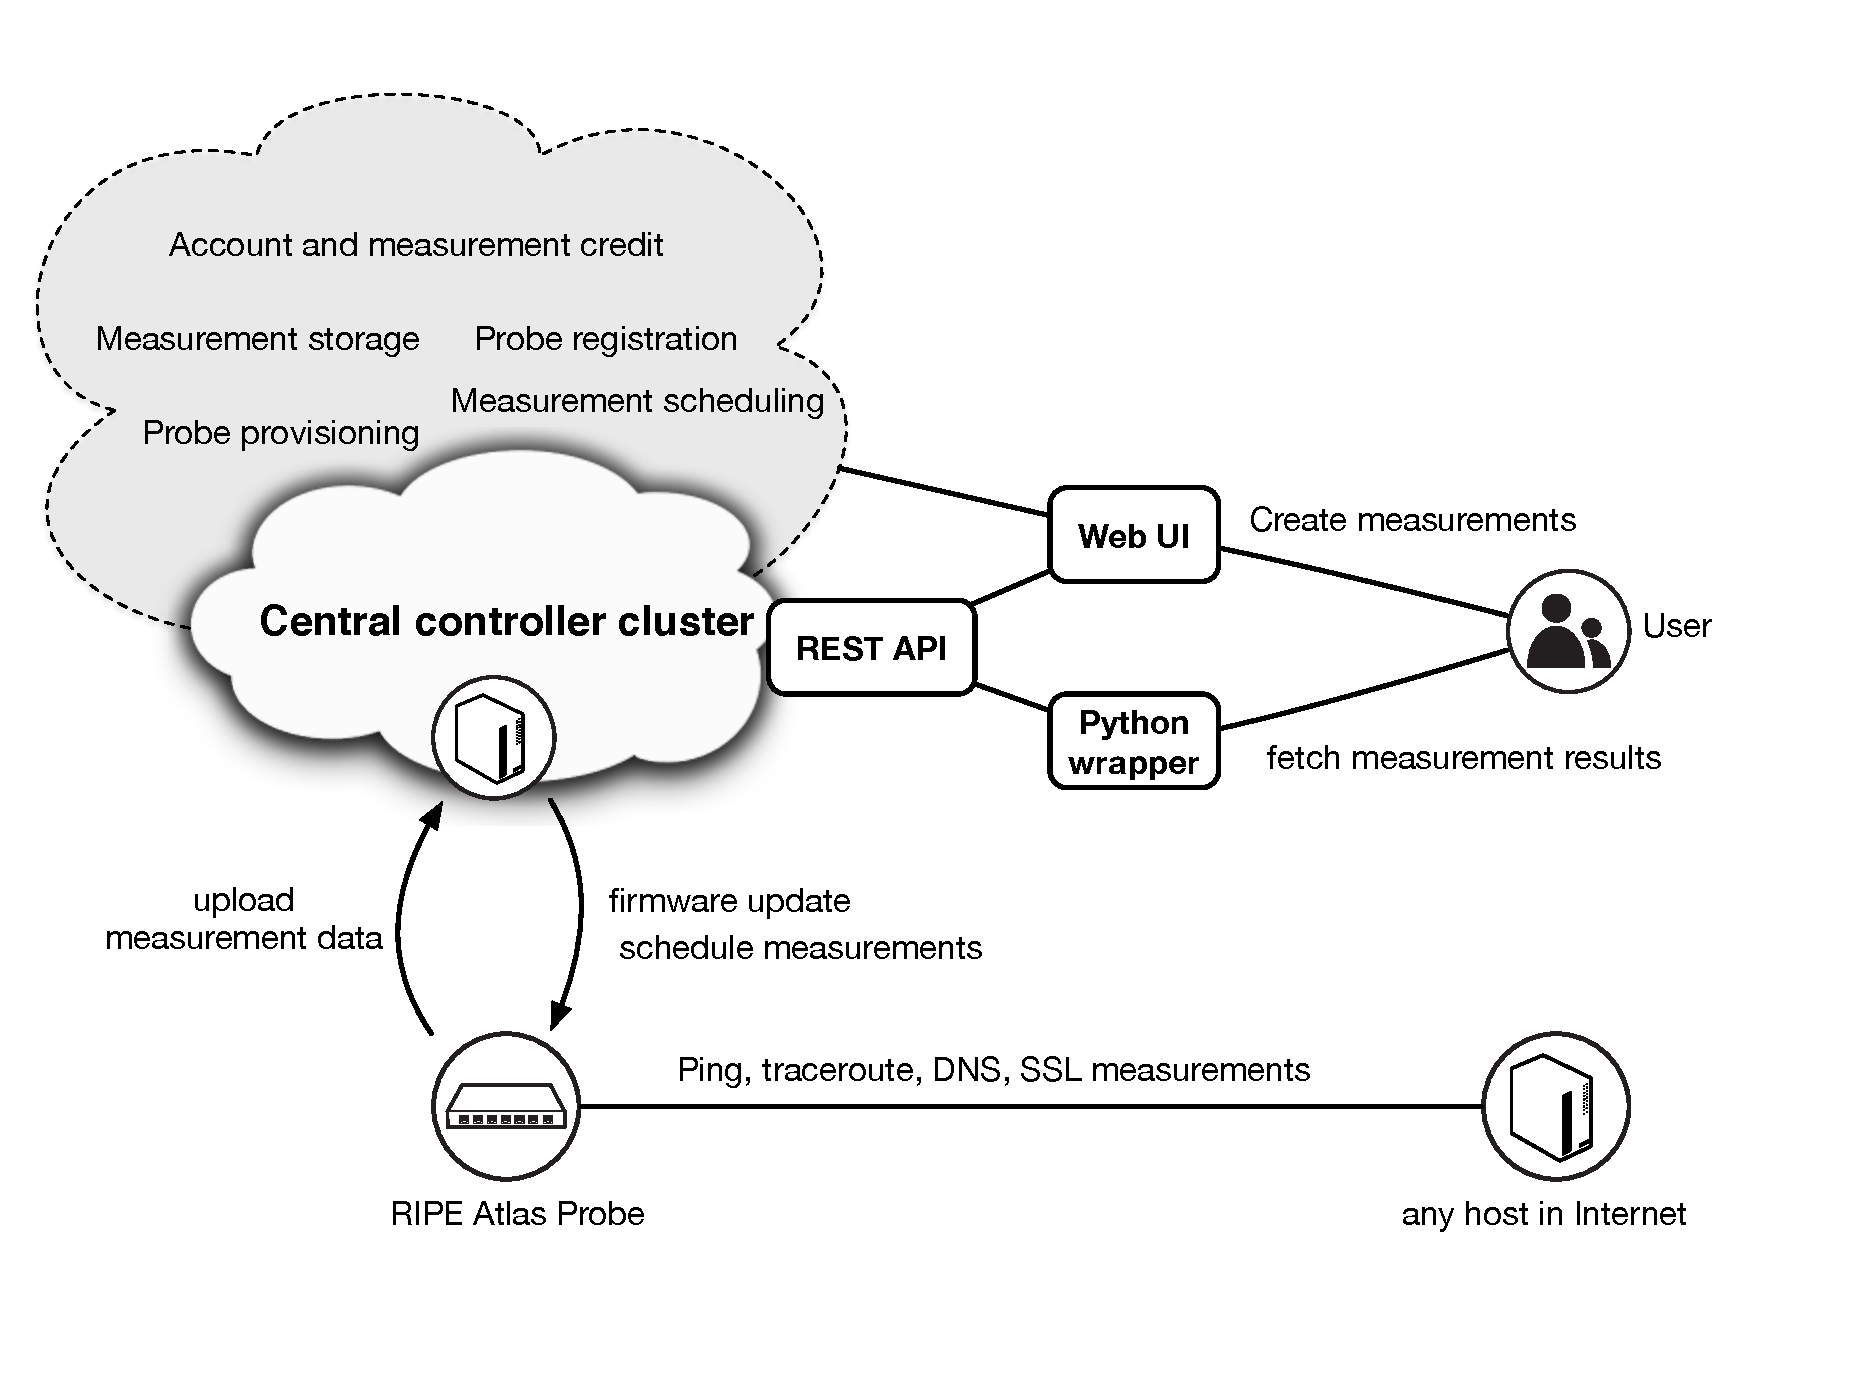
\includegraphics[width=\textwidth]{gfx/chap3/ripe_atlas_archi.pdf}
\caption{Building blocks of RIPE Atlas.}
\label{fig:ripe_atlas_archi}
\end{figure}

\acf{RIPE} Atlas is a measurement platform centrally managed by the European Internet register.
Fig.~\ref{fig:ripe_atlas_archi} sketches the architecture of the platform.
Probe are dedicated devices from which measurements are launched.
The operation system on the probes are tailored by RIPE engineers for Internet measurements~\cite{firmware}.
These probes are distributed either by RIPE or by RIPE Atlas Ambassador~\cite{ambassador} upon demand from anyone willing to host the probe and keep it online in his network.
As of this writing (July 11, 2017), 19448 probes have been sent out and 9854 of them remain active.
All these probes, hosted in 3511 IPv4 ASes and 1286 IPv6 ASes across 181 countries, can be commanded by a single platform user to measure any destination in the Internet.

As a platform user, one does not have to connect to all these probe by him/herself to 1) create specific measurements; 2) fetch measurement results. 
One only has to interface with RIPE to fulfill the above essential tasks along with other helpful functions such as measurement data visualization.
To that end, RIPE collects in quasi-realtime measurements from all the connected probes and stores them in its server clusters. Programming API~\cite{atlasapi} as well as human friendly Web sites are developed to facilitate the data operation of all kinds.

\subsection{Measurement types}
It is though not possible to run user specified measurement tools, e.g. nmnap~\cite{nmap}, scamper~\cite{luckie2010scamper} or bandwidth measurement tools, RIPE Atlas does support a wide range of standardized Internet measurements with configurable parameters: ping, traceroute, DNS, SSL.
Ping and traceroute measurement offer the Internet delay and path information required in measurement-based TE.

Another way of classifying the measurements is via the entity of measurement creator. As shown Fig.~\ref{fig:ripe_atlas_archi}, user of the platform (does not necessarily host probes) enjoys a great degree of 
liberty of specifying the destination and sources of supported measurements. These are \acf{UDM}. Once a user defines a measurement, the central controller clusters schedules it to corresponding probes and collects the results once the measurements started.
On the other hand, there exist another category of measurements defined by RIPE itself call built-in measurements~\cite{atlas}. These measurements are automatically executed by the probes themselves, with out need for controller commands. These measurements, originated from all probes, are mainly ping, traceroute and DNS measurements to DNS root servers and RIPE infrastructures.
In the later studies, we heavily rely on these built-in measurements given their world-wide footprint, super long history records (date back to the day one of each probe) and low additional measurement costs.

\subsection{Describe, identify and fetch measurements}
Besides measurement type specific parameters, such as the protocol type for traceroute, following three elements are as well fundamental describing a RIPE Atlas measurement: 1) participant probes; 2) the single measurement destination per measurement; 3) the time span of the measurement. 

Once a \ac{UDM} is created, it can be identified by a unique measurement ID. 
Each built-in measurement can as well be identified with a pre-assigned ID.
It is with this measurement ID, one learns the description, result visualization provided by RIPE and eventually fetches the raw measurement results.
For example, with \url{https://atlas.ripe.net/measurements/3742863/#!openipmap}, one can have access to the path visualization of measurement $\#3742863$, where 100 probes word-wide are selected to perform one-time traceroute toward \url{www.sigcomm.org}. With \url{https://atlas.ripe.net/api/v2/measurements/3742863/results/?start=1462147200&stop=1462233599&format=json}, anyone can easily download the entire raw measurement records of this measurement.

\subsection{Advantages}
RIPE Atlas is a measurement platform designed to facilitate reproducible researches. RIPE take care of all the engineering challenges of 1) measurements execution from geographically distributed probes; 2) reliable and continuous data storage; 3) public access to data; 4) simple syntax for describing, identifying measurements; 5) well documented open-source programming tools for data manipulation.

The advantages of RIPE Atlas go beyond reproducibility. Compared to perfSONAR, PlanetLab and DIMES, probes of RIPE Atlas, with dedicated hardware for measurement task, are supposed to deliver measurements better reflects the network character and less impacted by probe local resource sharing issues~\footnote{perfSONAR: ~\url{https://www.perfsonar.net}; PlanetLab:~\url{https://www.planet-lab.org}; DIMES:~\url{http://www.netdimes.org}}.
Moreover, thanks to its powerful monitoring capability, RIPE Atlas is gaining popularity among many non-academic networks, such as \ac{ISP} and \ac{CP}~\footnote{A monitoring use case by a online game company: \url{https://labs.ripe.net/Members/annika_wickert/using-ripe-atlas-to-monitor-game-service-connectivity}.}. Increasing number of these networks host RIPE Atlas probes or anchors (a more powerful version of normal probe),   providing a much richer and realistic network profile from which measurements can be initiated, compared to other alternative options.

\section{Measurement quality}
\subsection{Issue with RIPE Atlas}
We show that it is common to lose some datapoints for measurements scheduled at regular interval on RIPE Atlas. 
%Some hints on possible reasons are revealed by taking probe-to-controller connection activity into account.
The temporal correlation between missing measurements and connection events are %illustrated and 
analyzed, in the pursuit of understanding reasons behind such missings.
To our surprise, a big part of measurements are lost while probes are connected.

\subsection{Same AS path measured by different probes}
For multi-homed networks, inter-domain traffic engineering (TE) 
consists in selecting the best path available through the available transit providers,
so that the overall transmission quality is dynamically improved in front of network events, such as congestion and fail-over. 

In practice, the best next hop is chosen based on end-to-end (e2e) performance measurements toward destination networks. 
This requires reliable e2e measurements that estimate as accurately as possible inter-domain path characteristics, in particular Round-Trip Time (RTT).

These measurements usually prob
hosts with open ports, which are deliberately discovered in destination networks.
RTT traces so obtained can be affected by local factors, e.g. CPU load, that are not relevant for inter-domain routing and could thus mislead global route decisions. 

We data-mined the RTT time-series between two ASes with unsupervised learning method -- namely clustering.
%%%[TODO:] justify clustering method here
Achieved results show that our method is capable of improving measurement data quality, by excluding less reliable probes.
Moreover, we considered traceroute as well. 
Early results suggest that most variations of e2e delay actually occur in access networks. We thus believe that the proposed scheme can improve the accuracy and stability of the route selection for multi-homed networks.

\section{Synchronized RTT changes over different paths}
\label{sec:ripe_case_study}